%
\chapter{Introduction}\label{ch:background}
%

\section{Biological context and general questions}
	
	The work presented in this thesis revolves around several key biological concepts such as \emph{tissue}, \emph{cell type}, \emph{spatial coherency} and \emph{gene expression}. I define these notions in the Introduction and give an overview of the organism central to my work - \platyfull{}.\\
	
	The global goal of this thesis is to study single cell gene expression while taking into account the spatial context of each cell. My main contribution is the development of a method that demonstrates that taking into account the spatial information improves the clustering of single cells into functional tissues.\\
	
    The first written study of human anatomy that has survived through time and is sometimes attributed to Imhotep - physician, high priest and architect during the Old Kingdom of Egypt (3000-2500 BC) is the Edwin Smith Papyrus \citep{goodwin98,breasted30}. Although mainly descriptive, some organs such as the heart or blood vessels were defined functionally. A more scientific approach to anatomy based on animal and human dissections and vivisections arose in ancient Greece and was led by scientists such as Alcmaeon (510 BC),  Empedocles (480 BC) and later Aristotle (356 BC) \citep{singer57}. In these early studies the global \emph{function} of each organ was often inferred by analysing the result of accidental, war related or intentional injuries \citep{singer57}.\\ 
    
    As science developed and the scale of the smallest biological unit was reduced to the cell, organs were described as complex tissues: coherent structures composed of large numbers of cells. These cells are not identical to one another. First, visually, cells composing the tissue may have different physical characteristics. Second, when observing the cells in vivo, different cells in different parts of the complex tissue will exhibit different behaviour. Consequently, biological \emph{tissues} can be viewed as an interconnected mosaic of cells having different functions and working together to assume the global function of the tissue. When looking closely at this mosaic, it is sometimes possible to observe under a microscope \citep{young13} that the cells' spatial organisation is not random, thus leading to a classification of cells with respect to their appearance and behaviour. These categories are known as \emph{cell types}. Consequently, the definition of a complex biological tissue may be an ensemble of cells belonging to different cell types grouped in the same spatial structure.  If historically \emph{function} and physical characteristics of the organ were directly linked, microscopes and the observation of cells behaviour within a particular tissue changed this one to one relationship.\\
    
    The developing brain of the organism around which this thesis is built, \platyfull{} (presented in details in the next section), can be defined as a whole as being the central nervous system of the animal. This global functional definition encapsulates all the sub-functions of all the sub-tissues in the brain. For instance, when changing the scale of study from the organ to the tissue level, one can anatomically distinguish very different tissues (e.g photosentisive regions in the eyes and developing neurons).\\
    
    Interestingly, the cells making up specialized sub-tissues in the brain, belong to the same organ but have very different function. For example, photosensitive regions are composed of extremely specialized cells which display the ability to react to light stimulation \cite{arendt02} while developing neurons are part of the complex network that allows information to be transmitted and process in the brain \cite{Fischer10}.Importantly, as defined above, the brain has a coherent overall function, but when looking at the cell type level it is fascinating to observe that a wide variety of functions are displayed. Hence, my definition of a \emph{complex biological tissue} will be spatially coherent ensemble of cells organised in sub-tissues, each of which possesses a specific function.\\
    
     
    The sub-tissues in complex biological tissues tend to be spatially coherent. In other words cells that belong to the same cell type are usually structured spatially and as a result it seems sensible to assume that cells spatially close to one another have a greater probability of belonging to the same cell type. However, the spatial coherency of these sub-tissues is not always the same. Some cell types may consist of individual cells that are scattered inside another more spatially coherent tissue. An interesting example is the difference between the spatial coherency of cells forming the neuronal tissue in the brain and that of cells forming a well defined region in the brain like an exocrine gland. When asking the question: ``is it likely that this particular cell is fully surrounded by cells belonging to the same cell type?'', the extensions created by the axons of neurons (as shown in Figure \ref{fig:neuron}) will decrease this probability. Indeed, axons will grow through other types of tissues to reach their destination \citep{bartlett84,colello90}, making the overall spatial coherency of neural tissues smaller than very well spatially defined tissues.\\
    
\begin{figure}[bth]
\begin{center}
  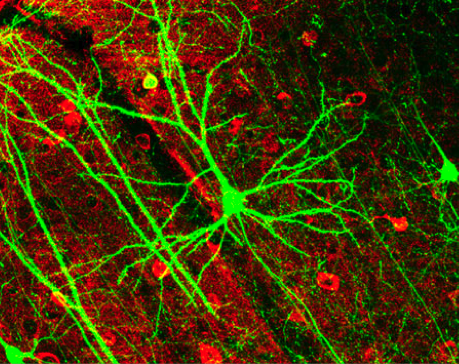
\includegraphics[width=0.8\linewidth]{gfx/chapter1/neuron.png}
\end{center}
  \caption{GFP staining of a pyramydal cell in mouse cortex showing dendrites and axons of a neuron linked and at the center the soma where the nucleus is located.In \platy{} the developed neurons display the same spatial characteristics. This Figure has been published under Creative Commons Generic license in \citep{lee06}.}
  \label{fig:neuron}
\end{figure}
	
     
    Organs and cell types have been defined mainly by their anatomical traits. However, the functional heterogeneity of complex tissues goes further than simple anatomical traits. In the case of the neurons presented above all display the same appearance in different parts of the brain as neuronal tissue makes up a good portion of the brain. However, looking closely at the function of the cells composing different parts of the brain composed of neurons unveils a completely different story. Indeed, despite their apparent similarity, some of them will for instance react to the neurotransmitter \emph{acetylcholin} while others will use \emph{glutamate} (example in the human brain \cite{hefti86,van93}, this difference is extremely important in terms of function.\\
     
     This very telling example shows that defining cell types based on their anatomical traits is clearly insufficient to characterize tissues.  As a result, I will now discuss a trait that fundamentally defines how cells are functioning, namely \emph{gene expression}. 

\section{Generalities about gene expression and development}\label{sec:gene_expression_background}     
       
     Throughout this thesis the term \emph{cell} will be used to refer to eukaryotic cells and, more specifically, those of multicellular organisms. Every cell in a complex organism possesses the same genome, that is, the sum of all the genetic information contained in the cell (nucleus and other compartments). This fundamental homogeneity is in plain contradiction with the heterogeneity observed anatomically. If every cell has the exact same DNA, where does the great variability between cell types come from? In other words, what makes a neuron become a neuron and not a pancreatic cell? Answering this type of question defines the field of developmental biology.\\
     
     A short answer to many developmental biology questions actually is: same genome but different pattern of gene expression. As a central cellular activity, numerous traits exhibited by cells throughout their life from their differentiation to their death, are defined by the way they express some specific parts of their genomes.\\

     To understand what gene expression is, the notion of \emph{gene} must first be defined. The precise definition of a gene remains controversial. The concept of a ``\emph{factor that conveys traits from parents to offspring}'' was laid down by Gregor Mendel in 1866 \citep{mendel66} when the accepted theory at the time was based on blending inheritance where the traits of the parents appeared mixed in the offspring following a continuous gradient. The most recently published definition of a gene followed the publication of the ENCODE project \citep{feingold04}. It states that a gene is ``\emph{a union of genomic sequences encoding a coherent set of potentially overlapping functional products.}''\\

	Gene expression describes the way cells express their genes. Expression of a gene is the process of transcribing the DNA of that particular gene. It is interesting to note that there are several ways to look at gene expression. Indeed in a cell or tissue, at a given time point it is possible to examine whether a gene is expressed or not (binary expression) or how much a certain gene is expressed (quantitative expression). The product of gene expression is RNA molecules. Technically speaking, for transcription to occur in the nucleus a complex system of proteins will attach itself onto the DNA double helix. In the case of protein coding genes, this complex is the RNA polymerase II. Once this complex becomes attached to the promoter region of the gene, transcription can begin. The RNA polymerase complex will move along the gene and replicate the template strand of the DNA in a process known as elongation. The resulting RNA molecule will be a copy of the coding strand of the DNA created by creating the complementary sequence of the template strand. When the polymerase reaches an ``end codon'', transcription terminates and the RNA molecule is released and polyadenylated in order to protect the transcript from degradation in the cytoplasm \citep{cooper00}.\\
	
	A portion of the RNA molecules are translated into proteins that can have very different purposes. Some will serve directly in the cellular life as functional/structural agents (elements of the ATP synthase for example \citep{boyer97}), others will be excreted by the cell and will serve a purpose at the scale of the organism \citep{kaiser84}. Others called transcription factors will have a regulatory effect on gene expression \citep{mitchell89}. In other words the expression of gene $G_a$, coding for protein $P_a$ might activate, accelerate, inactivate or decelerate the expression of gene $G_b$ and potentially others. This outlines the complex interdependent regulatory system that is gene expression, see Figure \ref{fig:cells}. For precise examples of gene regulatory networks, see \citep{gossen92, shinozaki03,fuqua01,balmer02}.\\
	
	
\begin{figure}[bth]
\begin{center}
  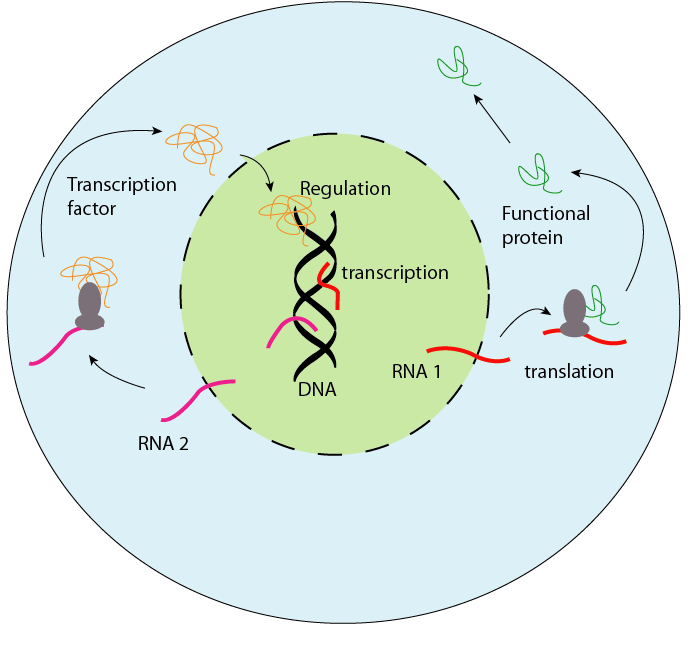
\includegraphics[width=0.8\linewidth]{gfx/chapter1/cell.png}
\end{center}
  \caption{Gene expression and protein translation and gene regulatory networks. The schematics shows that genes in the DNA are transcribed to RNA molecules that are further translated outside the nucleus into proteins. Those proteins can serve various purposes inside the cell or come back to the nucleus to regulate gene expression.}
  \label{fig:cells}
\end{figure}
	
	
	
	During development, different mechanisms exist that allow cells to develop differently from one to the other. This is how the asymmetrical axis (dorso-ventral, and basal-apical) of the body are defined. The main mechanisms for two cells to take two different differentiation pathways are signalling gradients and epigenetic control. They both act on the gene expression pattern of the cells. Epigenetic factors are directly coded onto the DNA structure but are not linked directly to the DNA sequence. Epigenetic modifications such as methylation or histone modifications influence gene expression by changing the accessibility of certain regions of the chromatin by modifying the chromatin state or the promoter strength \citep{jaenisch03}. Signalling gradients are environmental factors, they occur when cells grow in a medium containing certain chemicals. These chemicals will influence which gene they express \citep{chang02}. They can either penetrate the cells and directly regulate transcription as transcription factors \citep{durston89} or be recognized by some receptors at the surface of the cells that in turn will release transcription factors inside the cell \citep{wang92}. \\
	
	Consequently, gene expression is one of the key factors that drives tissue development. Therefore, the ability to study gene expression patterns has revolutionized the field of developmental biology. Technological innovation has been the main driving factor of this revolution and, in the next section, I will present two methods for assaying gene expression that are used throughout this thesis.


\section{Capturing gene expression in the laboratory}\label{sec:gene_expression_lab}
     \subsection{In-situ hybridization assays}
     In-situ hybridization (ISH) is an experimental technique where the practitioner is able to determine in which cells of the tissue under study a particular RNA is present. As opposed to Southern blotting \citep{southern75}, ISH assays not only enable the experimentalist to know whether a gene is expressed or not, but also where in the tissue it is expressed. First proposed in 1969 by Pardue \citep{pardue69} and John \citep{john69} independently, in-situ hybridization (ISH) used radioactive tritium labelled probes on a photographic emulsion to reveal parts of the studied tissues where particular RNA or DNA sequences were present.\\
     
      With the development of fluorescent labelling techniques \citep{landegent84,pinkel88} allowing for faster, more sensitive and of course safer hybridization assays compared to radioactive probes \citep{swiger96}, Fluorescent in-situ hybridization (FiSH) quickly became the standard technique to study gene expression in the spatial context of biological tissues. Importantly, using multiple fluorescent probes of different colours allowed the simultaneous localization of several RNA fragments within a tissue \citep{nederlof89}.\\
     
     For small enough tissues under study, it is possible to hybridize the probes in the whole animal. This method is called Wholemount in-Situ hybridization (WiSH) and a 3-Dimensional representation of the expression map of a gene can be deduced by using confocal microscopy to study the patterns of gene expression in the tissue slice by slice \citep{Tomer10}.
     

     \subsection{RNA sequencing}
     Whole Transcriptome Shotgun Sequencing (WTSS) also called RNA sequencing (RNA-seq) \citep{morin08,wang09} has developed alongside Next Generation Sequencing (NGS) techniques used to sequence genomic DNA. In RNA-sequencing, only the fraction of RNA molecules in the cell are targeted. Protein coding mRNA molecules can further be selected by isolating transcripts using their polyadenylated 3' tail, a characteristic exhibited by protein coding transcripts and a few other types of transcripts only (lncRNAs for example). Most current technique use magnetic beads to achieve this separation \citep{mortazavi08,morin08}.\\
     
    Once isolated from a population of cells, transcripts undergo fragmentation to obtain an average length of 200-300 nucleotides. The next step is the reverse transcription, which creates a complementary DNA (cDNA) library using viral reverse transcriptase enzymes. After amplification using quantitative Polymerase Chain Reaction (qPCR), the cDNA library is ready to be sequenced by NGS technology.\\
    
    NGS refers to numerous experimental techniques used to acquire the DNA sequences from a sample with a high throughput. I will not extensively describe all of these methods in this thesis but succinctly present some of them. 
    
\begin{itemize}
	
	\item 454 pyrosequencing \citep{margulies05} is a sequencing technique that revolves around luciferase binding, a light emitting protein, to detect and sequence the nucleotides while the complementary strand of single stranded DNA molecules are synthesised by DNA polymerase. The process of using DNA replication of single stranded DNA (ssDNA) molecules is referred to as \emph{sequencing by synthesis}. When the ssDNA molecule is entered in the sequencing machine, it is bound to the DNA polymerase using previously attached primer. The reaction is supplied with energy in the form of dATP$\alpha$S which does not react with the luciferase.\\
	
	One of the four possible denucleoside triphosphates (dNTP) is then added to the reaction. If the next nucleotide of the ssDNA strand to copy is complementary to the current dNTP, the DNA polymerase will catalyse the reaction, inserting the new nucleotide in the newly created strand and realising an inorganic phosphate (PPi). The enzyme ATP sulfurylase added to the reaction will transform the PPi in ATP which will in turn react with the luciferase and emit light, signalling that the base complementary to the current dNTP was the next nucleotide of the ssDNA.\\
	
	If two or more nucleotides added at the same time (in the case of nucleotide repetition), this can be detected by analysing the intensity of the emitted light which is proportional to the number of PPis released. Repeating this procedure in turn for each dNTP until the whole ssDNA has been replicated allows the sequence to be fully determined.
	
	\item Illumina sequencing \citep{bentley08} is one of the most commonly used NGS technology. Similarly to 454 pyrosequencing, light emission is used through dyes to detect the nucleotides of ``DNA colonies''. During the library preparation step, the double stranded DNA is fragmented and the sheared ends are repaired and adenylated. Adaptors are then bound to each end of the fragments which are subsequently size selected and purified.\\
	
	 The next step is cluster generation where single DNA molecules are isothermally amplified to prepare them for sequencing. To this end, the adaptors ligated to the DNA molecules are bound on a surface with numerous oligo primers. Once the ssDNA molecules are bound from one end to the surface, the DNA strand is copied and ssDNA copies are bound to the surface on the other end as well, creating bridges. These bridges are amplified through a process know as isothermal bridge amplification resulting in millions of ``DNA clusters''. The bridges are destroyed on one side and sequencing primers are then hybridized on the free end of the ssDNA molecules.\\
	 
	 Finally the DNA clusters can be sequenced. Each fragment is sequenced base by base, by adding the four possible denucleoside triphosphates (dNTP), each bound to a different fluorescent marker. The dNTP will compete with each other to bind to the DNA template which means that the dNTP complementary to the current DNA nucleotide is very likely to be incorporated. Once the non-reacting dNTP fragments are washed away, the clusters are excited by a laser emitting a light with a specific frequency that identifies the newly added base. The fluorescent block is then removed and the sequencing cycle is repeated until the complete fragment has been sequenced.
    
\end{itemize}     
    
    The described sequencing methods generate large datasets of short reads, which need to be mapped back to the reference genome of the considered species, providing this genome is available. In this case, the resulting dataset will reflect a snapshot of the whole transciptome in the studied cell population. In the case where the reference genome is not fully available, an alternative option is to map the reads back to a list of known gene sequences. The resulting dataset will represent a quantitative image of the considered genes in the cell population at one point in time.\\
    
    Because of technical limitations in these sequencing protocols, until very recently the starting quantity of RNA was relatively important (this issue is discussed further in \ref{sec:single_cell_rnaseq}). This is why most of the published RNA sequencing studies use a population of cells as a starting point. This, however, means that the gene expression landscape obtained as an output will represent an averaged expression over all the cells used as an input.\\
    
    Importantly, when comparing RNA-seq to the previously described in-situ hybridization technique, while the methodological burden for analysing the expression of many genes at the same time is greatly reduced, the spatial localisation of the cells is lost during the protocol.\\
    
    At this point I have defined some methods to study gene expression and why this information is crucial to understand the mechanisms of developmental biology. Experimentally speaking, biological studies rely upon numerous model organisms such as \species{Mus musculus}, \species{Caenorhabditis elegans}. The work presented in this thesis revolves around the marine annelid \platyfull{}. In the next section, I will introduce generalities about this interesting model organism and in particular how its neural system is ideal for studying brain development and evolution.
    
    
\section{Platynereis dumerilii, an ideal organism for studying brain evolution}\label{sec:platynereis}
     \subsection{General description}
     \platyfull{} is a marine annelid of the class Polychaeta, which has been established as one of the main marine animal models in the fields of evolutionary, and developmental biology as well as ecology, toxicology and neurobiology \citep{hutchinson95,tessmar03,hardege99,dorresteijn90,fischer04,Fischer10}.\\
     
     \platy{} populates shallow (no more than 3m deep) ocean floors around the world. It is commonly found in the Mediterranean sea, the north Atlantic coast of Europe as well as in the shallow seas surrounding Sri Lanka, Java and the Philippines. Eggs, embryos and larvae are roughly 160$\mu$m long while the adults can measure up to 6cm in length.
     
     
\begin{figure}[bth]
        \myfloatalign
        \subfloat[Larval form of \platy{}. Image: MPI for Developmental Biology.]
        {\label{fig:platynereis_larvae}
        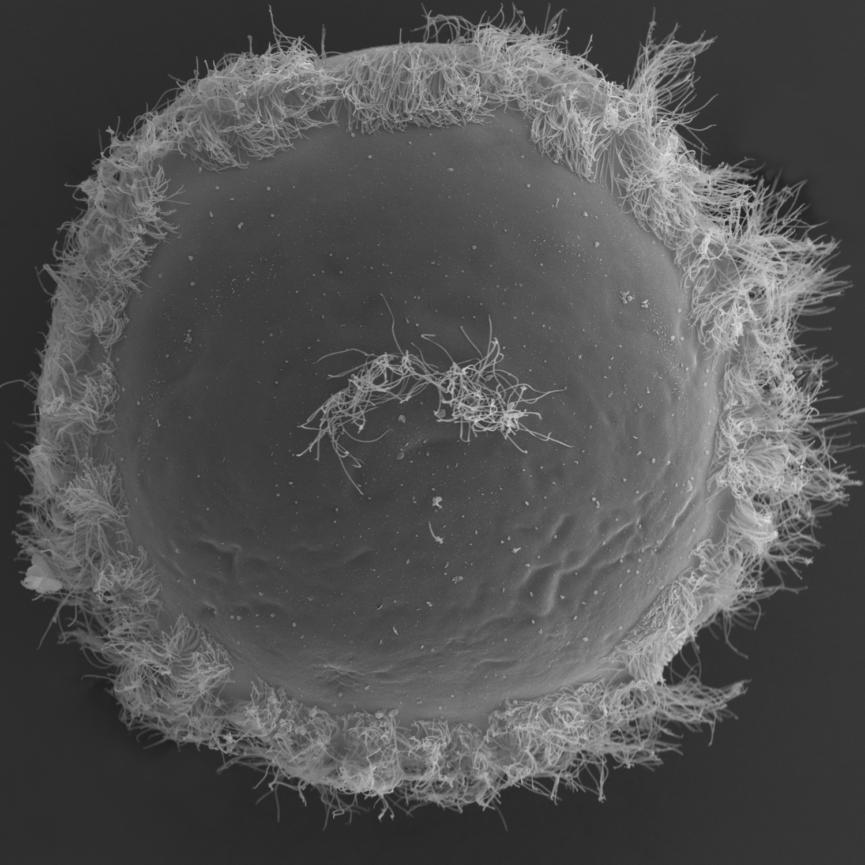
\includegraphics[width=.45\linewidth]{gfx/chapter1/platynereis_larva.jpg}} \quad
        \subfloat[Adult \platy{}. Image: Arendt group, EMBL]
        {\label{fig:platynereis_adult}%
         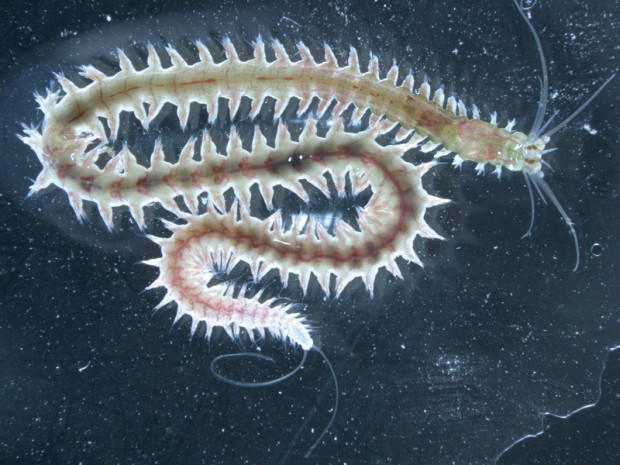
\includegraphics[width=.45\linewidth]{gfx/chapter1/platynereis_adult.jpg}}
        \caption{\platyfull{}'s larva and adult forms.}\label{fig:platynereis}
\end{figure}
     
     There are several reasons why \platy{} has been chosen as a model by numerous laboratories. Indeed, evolutionary wise, \platy{} shows several interesting characteristics.  As a member of the bilaterians \platy{} has a defined bilateral symmetry. It belongs to the lophotrochozoan taxon of the bilaterians as opposed to most of the well established model animals which either belong to the ecdysozoans (\species{Caenorhabditis elegans}, \species{Drosophila melanogaster}) or the deuterostomes (mouse, human). \platy{}, as one of the only lophotrochozoan models is needed in order to use comparative approaches for studying the full range of bilaterians \citep{Fischer10}.\\
     
     \platy{} also exhibits an exceptionally slow evolving nature and it has even been described as a ``living fossil'' for that reason \citep{Fischer10}. Consequently, the numerous ancestral developmental characteristics of \platy{} partly reflect the common ancestor of all bilaterians. An interesting example described in \citep{denes07,tessmar07} is the conserved molecular topography of the genes responsible for the development of the central nervous system between \platy{} and all vertebrates. This slow evolving nature makes \platy{} a better comparison with vertebrates than fast evolving species like \emph{Drosophila} and nematodes where derived features can obscure evolutionary signal \citep{Fischer10,arendt124}.\\
     
     Experimentally speaking, model organisms are chosen for several characteristics that make them easy to use in the laboratory. These characteristics include, but are not limited to, the size of the animal, the conditions required for the organism to develop, gestation and development time as well as the ease with which a new generation can be produced.\\
     
     In this regard \platy{} is nearly an ideal animal. Even in their adult form, they are relatively small, they can easily be kept and bred in captivity producing offspring throughout the year \citep{fischer04}. Furthermore, the behavioural characteristics of \platy{}'s mating ritual have been well studied and can be reproduced on demand in the laboratory. The ``nuptial dance'' happens on the water surface. Males and females respectively release the sperm and eggs synchronously. This activity is synchronized by pheromones released into the water \citep{zeeck98}. Over 2000 individuals can be produced within a single batch. Every new individual will undergo embryonic then larval development before reaching \platy{}'s adult form.\\

 
     \subsection{Larval development}
    Similarly to the other polychaetes, the larval development of \platy{} can be decomposed into three main anatomical stages, as detailed in \citep{hauenschild69}: the trochophore, the metotrochophore and the nectochaete. The trochophore is spherical and moves thanks to an equatorial belt of ciliated cells as well as an apical organ displaying a ciliary tuft \citep{rouse99,nielsen04} as seen in Figure \ref{fig:platynereis_larvae} and schematically in Figure \ref{fig:platynereis_larvae_scheme}. The metotrochophore stage is characterized by the development of a slightly elongated segmented trunk compared to that of the trochophore \citep{hacker98}. The next developmental stage is referred to as the nectochaete larvae which resembles the adult (figure \ref{fig:platynereis_adult}) in many traits, especially with parapodial appendages used for swimming and crawling \citep{hacker98}.\\
    
\begin{figure}[bth]
\begin{center}
  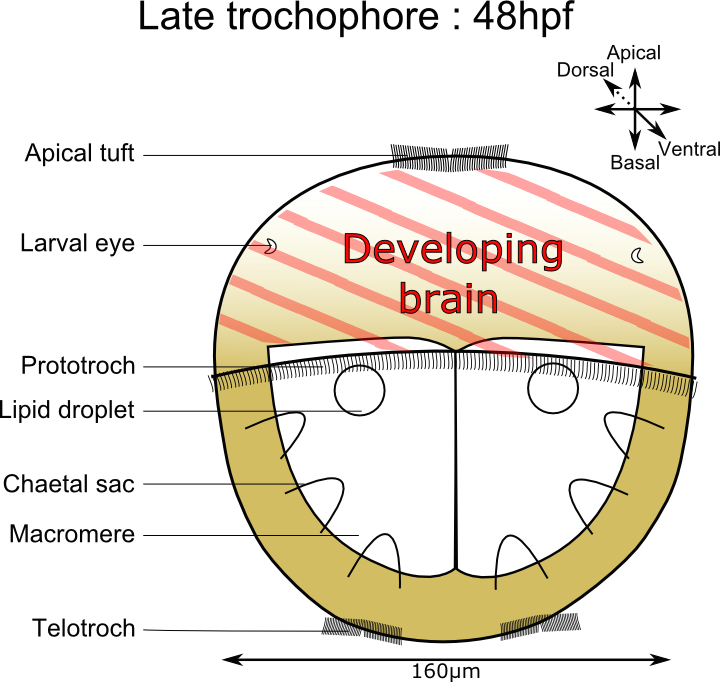
\includegraphics[width=\linewidth]{gfx/chapter1/larvae48hpf.png}
\end{center}
  \caption{\platyfull{}'s larvea development at 48hpf (late trochophore). Red stripes indicate the area that forms the developing brain of the larvae.}
  \label{fig:platynereis_larvae_scheme}
\end{figure}
    
    Aside from this purely anatomical description, an additional staging system exists and has become the norm for current studies. The development is measured in \textit{hours post fertilization} (hpf) at $18^{\circ}C$.
    
    A key factor making \platy{} such an interesting model to work with is the fact that after fertilization, the $\approx 2000$ larva will start developing at the exact same time, in a synchronous fashion. Furthermore, the larval development of \platy{} follows a very stereotypical pattern with little variation from one individual to the other; this is true even between batches provided the temperature is kept constant \citep{fischer04,dorresteijn90}. An illustration of this synchronous development is shown in Figure \ref{fig:brain_comparison}. This is a very important feature as it allows biologists to repeat experiments on several individuals at a very close developmental stage even if they are from different batches.\\
    
\begin{figure}[bth]
  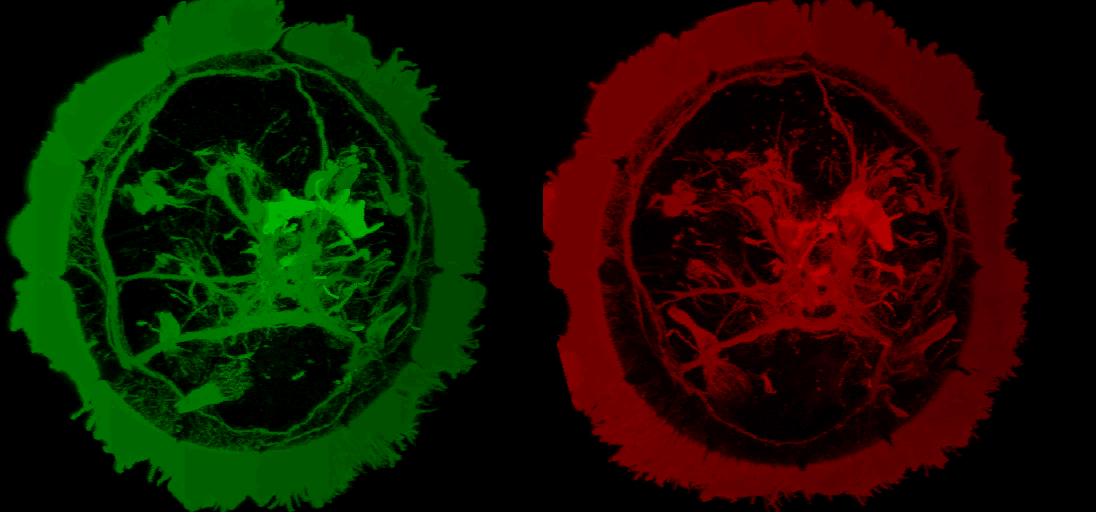
\includegraphics[width=\linewidth]{gfx/chapter1/brain_comparison.png}
  \caption{\platyfull{}'s stereotypical and synchronous development. In green and red are two different \platy{} individuals' with the same gene expression being highlighted. They show extremely similar patterns of development for the nervous system.}
  \label{fig:brain_comparison}
\end{figure}

	 
	  \subsection{Platynereis' nervous development until 48hpf}
	 Describing the entire development of \platy{} does not fall within the scope of this thesis. Indeed, I will only be interested in the brain of \platy{}'s larvae at 48hpf. Therefore, it is important to have an anatomical idea of what the brain looks like at this time in development and what inherent characteristics will be the most interesting to investigate. \platy{}'s larval brain development is detailed in \citep{Fischer10}.\\
	 
     From the early trochophore (24-26hpf) neural system development starts taking place. The apical ganglion which contains one sertonergic cell and a few neurons linked to the nerve of the ciliary band of the larva called the prototroch forms at the apical tuft, (see Figure \ref{fig:platynereis_larvae_scheme}). This allows the first movements of the larvae thanks to the cialited cells of the prototroch.\\
     
     The mid-trochophore (26-40 hpf) sees the formation of the first cerebral commissure: a band of nerves interconnecting the ventral nerve cord and the brain, which is a typical feature of annelid neurobiology. During this phase the apical ganglion becomes bigger with three more serotonergic cells.\\
     
     The late trochophore (40-48hpf) sees the formation of the second commissure in the ventral nerve cord. It is at the end of this stage that the tissues of the brain become more complex with a notable increase in the number of neurites \citep{Fischer10}.\\
     
     The data used in the rest of this thesis will not encapsulate the whole larvae, just the developing brain (see Figure \ref{fig:platynereis_larvae_scheme}) thus excluding the ventral part of the nervous system. The best studied areas of the developing brain are the larval eyes, the developing adult eyes and the apical organ on the dorsal side. On the ventral side are located the mushroom bodies, a pair of structures that are known to play a role in olfactory learning and memory in insects and annelids \citep{Tomer10}.\\
     
     Consequently, even at this early stage in a relatively ``simple'' organism, the brain quickly becomes an extremely complex tissue. Cell types diverge and functional areas are formed. Before trying to understand more about \platy{}'s brain organization, it is interesting to ask the more general question of how complex tissues such as the brain are defined spatially.


    
\section{Summary}
     
     

	In the introduction, I have presented a central aspect of cell and developmental biology, namely, gene expression. I have given an overview of how cells express their genomes and how the expression of specific signalling genes can influence the fate of cells during development. I have also described two methods that allow practitioners to capture gene expression from a biological tissue: in-situ hybridization and RNA-seq.\\
	
	Subsequently, I described \platyfull{} and the advantageous traits it exhibits for developmental biologists especially in the field of neural development. I have discussed the fact that anatomical traits are not sufficient to fully comprehend the deep heterogeneous patterns of functionalities inside a complex organ such as the brain. In order to push this understanding further I have discussed how gene expression levels can be used to characterise different tissues and how an image library of gene expression for 169 gene was generated by \citep{Tomer10} in the full brain of \platy{} using WiSH.\\
	
	So far, I have considered biology at the scale of the tissue, or the sub-tissue. However, the heterogeneity of complex biological tissues does not stop at this scale of study. In fact, with a top-down approach looking at big tissues and then separating them in smaller sub-tissues until ``true'' functional tissues are defined is an extremely complicated problem. A solution to this problem would be to reverse the approach from a top-down to a bottom-up mindset. This means reducing the scale of study to the smallest biological unit available, the single cell, defining the heterogeneity of gene expression at the single cell level and going back up to the functional tissue level from there. Instead of a fragmentation problem, this becomes a clustering problem, attaching single cells to a certain number of categories. In order to implement such an approach, single cell gene expression data is therefore needed.\\
	
	This model animal, the image library of gene expression in its brain and the question of finding functional tissues and sub-tissues from single cell gene expression are the key concepts that motivate this thesis.\\
	
	In Chapter \ref{ch:singlecell}, I describe how advances in both RNA-seq and in-situ hybridization have allowed the extraction of single cell gene expression data and how this data is analysed. I also describe how an ``ideal'' dataset of spatially referenced single cell expression data can potentially be created by mapping the results of single cell RNA-seq onto an in-situ hybridization scaffold.\\
	
	In Chapter \ref{ch:non_spatial_clustering_visualization} I present a tool I developed to allow an easy visualization of 3D information and more specifically clustering results. This tool is central to the upstream and downstream analysis of the data and the results used in the thesis.\\
	
	In Chapter \ref{ch:HMRF} I  present the theoretical background underlying the Hidden Markov random fields (HMRF) spatial clustering method I developed and how this method diverges from previously described HMRF methods. \\
	
	I then evaluate in Chapter \ref{ch:simulations} the performances of the HMRF method on simulated data. I describe how binarized gene expression data with a spatial component was simulated, then validate the parameters estimation by the method and finally compare the performance of the method to other non spatial clustering methods in terms of clustering quality and computing resources.\\
	
	I present in Chapter \ref{ch:biology} the results of the HMRF method when applied to the binarized single cell in-situ hybridization data in the brain of \platyfull{}. First, I propose a scoring method in order to use the clustering results to functionally define the regions. I then validate the method further by describing known regions of the brain that are found by the method. Finally I discuss how functional hypothesis can be made for unstudied regions of the brain.
	
	
	

%
%
%
%
%



